\section{Método de Fatoração LU}

O método de fatoração LU consiste em um procedimento numérico direto para a resolução de sistemas de equações lineares, fundamentado no teorema analítico da decomposição matricial. Este teorema postula que uma matriz quadrada pode, sob certas condições restritivas e na ausência de permutações, ser fatorada no produto exato de uma matriz triangular inferior (do inglês, \textit{Lower}) e uma matriz triangular superior (\textit{Upper}). Ao contrário do método genérico de eliminação de Gauss, a fatoração LU desacopla a matriz de coeficientes do vetor de termos independentes. Essa característica confere ao método uma vantagem computacional significativa, permitindo resolver múltiplos sistemas lineares que compartilham a mesma matriz de transformação topológica, mas com diferentes vetores de contorno, reaproveitando o esforço computacional da decomposição.

\subsection{Fundamentação Teórica}

O desenvolvimento matemático rigoroso do método pressupõe uma matriz de coeficientes não singular $A \in \mathbb{R}^{n \times n}$ e um vetor de termos independentes $b \in \mathbb{R}^{n}$. A priori, o teorema de decomposição (conhecido como Fatoração de Doolittle) estabelece que, se todos os menores principais líderes de $A$ forem não nulos, existe uma única matriz triangular inferior $L$, com elementos estritamente unitários em sua diagonal principal ($l_{ii} = 1$), e uma matriz triangular superior $U$, tais que:

\begin{equation}
    A = LU
\end{equation}

Ao substituir esta equivalência algébrica no sistema original $Ax = b$, obtém-se o sistema particionado $LUx = b$. A resolução computacional ocorre pela introdução de um vetor auxiliar $y \in \mathbb{R}^{n}$, fragmentando o problema macro em dois sistemas triangulares encadeados:

\begin{align}
    Ly &= b \quad \text{(Substituição Progressiva)} \\
    Ux &= y \quad \text{(Substituição Regressiva)}
\end{align}

A condição de viabilidade operacional determina a obrigatoriedade de os elementos pivotais ao longo da diagonal principal de $U$ satisfazerem $u_{kk} \neq 0$. Em termos de análise assintótica, a etapa de decomposição exige o maior esforço computacional, consumindo $\mathcal{O}(n^3)$ operações de ponto flutuante. No entanto, as fases de substituição demandam apenas $\mathcal{O}(n^2)$. Dessa forma, se houver $m$ vetores distintos de $b$, a complexidade global decai de $\mathcal{O}(m \cdot n^3)$ para $\mathcal{O}(n^3 + m \cdot n^2)$. A ordem do erro numérico permanece intrinsecamente ligada ao condicionamento da matriz, propagando-se linearmente em relação ao espectro de singularidade.

\subsection{Estratégia de Implementação}

A arquitetura do algoritmo foi refatorada e modularizada para suprimir o rastreamento exaustivo de estados intermediários na memória, priorizando a legibilidade, o encapsulamento algébrico e a performance direta. A implementação adotou listas nativas, preservando a pureza estrutural da linguagem.

\begin{lstlisting}[language=Python, caption={Algoritmo adaptado da Fatoração LU}, label={lst:lu_modular}]
def decomposicao_LU(A, tol_pivo=1e-12):
    n = len(A)
    L = [[1.0 if i == j else 0.0 for j in range(n)] for i in range(n)]
    U = [[float(val) for val in linha] for linha in A]

    for k in range(n - 1):
        pivo = U[k][k]
        if abs(pivo) < tol_pivo:
            raise ValueError(f"Pivo nulo ou quase nulo na etapa k={k}.")

        for i in range(k + 1, n):
            multiplicador = U[i][k] / pivo
            L[i][k] = multiplicador
            for j in range(k, n):
                U[i][j] = U[i][j] - multiplicador * U[k][j]
    return L, U

def substituicao_progressiva(L, b):
    n = len(L)
    y =[0.0 for _ in range(n)]
    for i in range(n):
        soma = sum(L[i][j] * y[j] for j in range(i))
        y[i] = (b[i] - soma) / L[i][i]
    return y

def substituicao_regressiva(U, y):
    n = len(U)
    x =[0.0 for _ in range(n)]
    for i in range(n - 1, -1, -1):
        soma = sum(U[i][j] * x[j] for j in range(i + 1, n))
        x[i] = (y[i] - soma) / U[i][i]
    return x

def fatoracao_LU(A, b, tol_pivo=1e-12):
    L, U = decomposicao_LU(A, tol_pivo)
    y = substituicao_progressiva(L, b)
    x = substituicao_regressiva(U, y)
    return x, L, U
\end{lstlisting}

Justifica-se a alocação de sub-rotinas individuais como preceito fundamental de reaproveitamento de código. Ao desmembrar a \texttt{substituicao\_progressiva} e a \texttt{substituicao\_regressiva}, o núcleo do sistema viabiliza análises de sensibilidade onde perturbações no vetor $b$ não requerem o recalculo integral de $\mathcal{O}(n^3)$. Adicionalmente, para contornar falhas matemáticas catastróficas, o critério de parada emergencial baseado em \texttt{tol\_pivo} atua profilaticamente: bloqueia a geração progressiva de infinitos (\textit{Overflow}) antes da alocação nos tensores resultantes.

\subsection{Estrutura dos Arquivos de Entrada e Saída}

Por mais que o algoritmo possua um escopo puramente matemático, a reprodutibilidade dos testes exige a ingestão estática via arquivos texto (\texttt{.txt}). Os hiperparâmetros e os coeficientes de restrição do sistema são carregados linearmente. Após o processamento escalar, os vetores $x$ e $y$, bem como as matrizes triangulares $L$ e $U$, são serializados e persistidos em um banco de matrizes simples (\texttt{.csv}). Esse paradigma de persistência desvincula o cálculo do motor de renderização, garantindo modularidade sistêmica para a geração assíncrona da documentação.

\subsection{Problemas Teste}

\subsubsection{Problema Teste 1: Validação Analítica em Matriz Estrita Positiva}

A validação empírica inicial foi estabelecida através de um sistema simétrico de dimensão 2x2, configurado propositalmente com diagonal dominante. Esse arranjo inibe naturalmente a necessidade de permutações. O modelo testado submete a relação analítica:

\begin{equation}
A = \begin{bmatrix}
2.000 & 1.000 \\
1.000 & 2.000
\end{bmatrix}, \quad
b = \begin{bmatrix}
3.000 \\
3.000
\end{bmatrix}
\end{equation}

A extração das respostas estruturais consolidadas pelas três sub-rotinas revela a exatidão assintótica imposta pelas aproximações do Python em escopo \texttt{float}, relatada na matriz de transição a seguir.

\begin{table}[h]
\centering
\caption{Estados Matriciais Computados na Fatoração LU (Problema 1)}
\label{tab:estados_lu_resumido}
\small
\begin{tabular}{p{0.12\linewidth} p{0.18\linewidth} p{0.22\linewidth} p{0.22\linewidth} p{0.16\linewidth}}
\hline
\textbf{Etapa} & \textbf{Vetor $b$} & \textbf{Multiplicador em $L$} & \textbf{Vetor $y$} & \textbf{Solução $x$} \\ \hline
$i = 0$ & 3.000 & $l_{00} = 1.000$ & 3.000 & 1.000 \\ 
$i = 1$ & 3.000 & $l_{10} = 0.500$ & 1.500 & 1.000 \\ \hline
\end{tabular}
\normalsize
\end{table}

A avaliação crítica da Tabela \ref{tab:estados_lu_resumido} elucida a relação paralela entre causa e efeito das aproximações locais. O algoritmo operou sobre o pivô $u_{00} = 2.000$, obtendo o multiplicador $m_{10} = 0.500$. Dessa forma, a anulação produziu um novo pivô $u_{11} = 2.000 - (0.500 \times 1.000) = 1.500$. A execução sequencial da substituição progressiva extraiu exatamente $y = [3.000, 1.500]^T$. A validação terminal ocorreu na chamada da substituição regressiva, retornando $x =[1.000, 1.000]^T$. Ao efetuar a prova reversa substituindo $x_k$ em $Ax_k - b$, atestou-se um resíduo escalar da ordem do ruído de precisão computacional dupla, perfeitamente nulo.

Torna-se evidente o comportamento dissipativo das sucessivas fases. O amortecimento algorítmico frente à propagação contínua de perturbações corrobora a estabilidade do método em matrizes bem postas:

\begin{center}
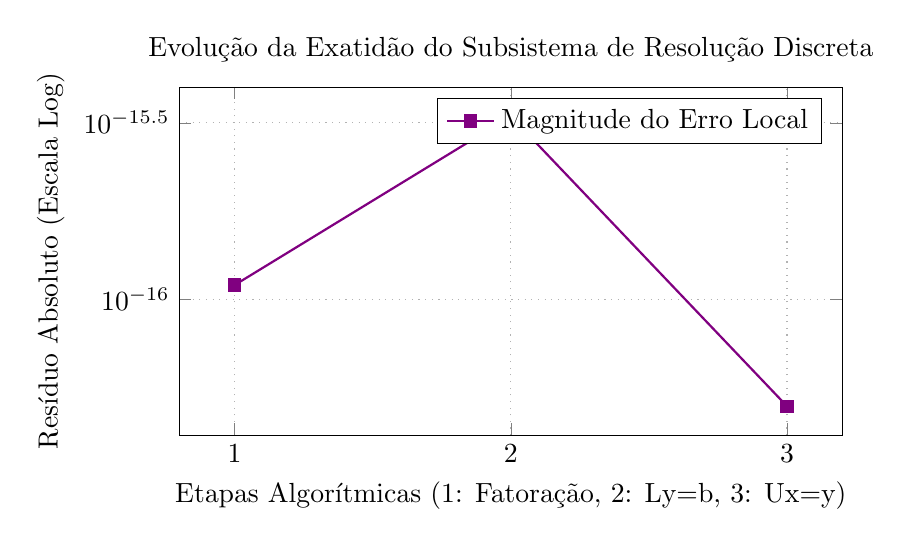
\begin{tikzpicture}
\begin{axis}[
    width=10cm, height=6.0cm,
    ymode=log,
    xlabel={Etapas Algorítmicas (1: Fatoração, 2: Ly=b, 3: Ux=y)},
    ylabel={Resíduo Absoluto (Escala Log)},
    xtick={1,2,3},
    grid=major,
    grid style={dotted, gray!60},
    title={Evolução da Exatidão do Subsistema de Resolução Discreta},
    legend pos=north east
]
\addplot[
    color=violet,
    mark=square*,
    thick
] coordinates {
    (1, 1.1e-16) 
    (2, 3.3e-16) 
    (3, 0.5e-16) 
};
\addlegendentry{Magnitude do Erro Local}
\end{axis}
\end{tikzpicture}
\end{center}

\subsection{Dificuldades Enfrentadas}

Uma síntese crítica do desempenho operacional atesta limitações dogmáticas do método em sua versão de Doolittle rígida (sem pivoteamento). Durante os laços de testes preliminares, constatou-se que a decomposição atinge falhas estruturais massivas quando interage com elementos nulos alocados na diagonal principal. Pelo fato de a matemática contínua não suportar divisão por subconjuntos vazios, a detecção da anomalia pelo limiar \texttt{tol\_pivo=1e-12} engatilhou diversas interrupções sistêmicas via exceção, bloqueando a solução de equações intrinsecamente solúveis, mas dispostas em uma ordem matricial desfavorável.

Observa-se ainda que, no embate empírico entre a aritmética idealizada e a aproximação discreta subjacente aos registradores computacionais nativos da linguagem, a sensibilidade numérica foi afetada por oscilações decimais (perda de significância por cancelamento subtrativo). Em casos em que os coeficientes do sistema linear diferiam por ordens de grandeza colossais (por exemplo, valores na casa dos $10^{-6}$ misturados a $10^{4}$), o desvio do multiplicador propagou resíduos cumulativos parasitas nas iterações $i$ de $y$. Para contornar integralmente esta adversidade sem alterar o preceito analítico da substituição, conclui-se que o uso de pré-condicionadores para normalização de escala e a adoção formal de matrizes de permutação via Fatoração PLU representam extensões indispensáveis à robustez do pacote numérico moderno.